\section{Related work}
\subsection{Built-in spreadsheet tools}
\label{sec:built-in-tools}
Excel and LibreOffice Calc have their own built-in tool to track dependents and precedents of a cell. If a user tracks for example the precedent of a cell (figure~\ref{fig:precedent-libre}), the program draws an arrow of the precedent to the cell. Even though the arrows highlight the precedent / dependents of a cell, if they are located on a different worksheet the user has to move to the other worksheet and possibly lose their current spatial context. Another issue is that the user only sees the precedents / dependents which are in the viewport. If they are not located in the current viewport the user has to scroll away to locate the precedents / dependents.
\begin{figure}[H]
    \centering
    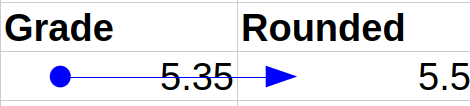
\includegraphics[scale=0.3]{chapters/methods/images/precedent-tracking-libre.png}
    \caption{Tracking a precedent of a cell in LibreOffice Calc}
    \label{fig:precedent-libre}
\end{figure}

\subsection{Separate dataflow visualizations}
\subsubsection{Leveled dataflow}
\label{sec:leveled-dataflow}
Several studies have proposed different approaches to display the underlying dependency graph of spreadsheets. 
Hermans et al. present in their paper \textit{Supporting Professional Spreadsheet Users by Generating Leveled dataflow Diagrams}~\cite{hermans_supporting_2011}, a solution to explicitly show these relationships. Their approach consist of three Views: The global view, the worksheet view and the formula view. The global view (figure~\ref{fig:global-view}) shows the relationships between the worksheets. The worksheet view groups the data in a worksheet into blocks and how they relate to each other. On the lowest level is the formula view which gives more detail about the calculations of a specific formula. One of the limitations of the leveled dataflow is that it is a read only tool. It does not exist bidirectionality to allow the user to connect the data blocks to the data in the worksheet. Unlike the multiple representation spreadsheet discussed below, it does not allow edits to the view.
\begin{figure}
    \centering
    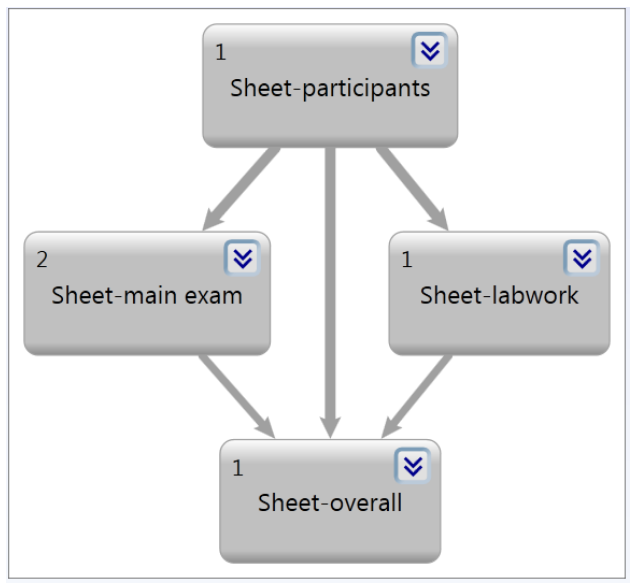
\includegraphics[scale=0.3]{chapters/methods/images/global-view.png}
    \caption{An example global view \cite{hermans_supporting_2011}}
    \label{fig:global-view}
\end{figure}

\subsubsection{Multiple representation spreadsheet}
\label{sec:multiple-representation}
To tackle the inability to clearly see the underlying computational structure and lack of abstraction, Sarkar et al. present their solution, multiple representation spreadsheet, in the paper \textit{Calculation View: multiple-representation editing in spreadsheets}~\cite{sarkar_calculation_2018}. Their solution leaves the grid and formula syntax untouched, but it should provide additional representation to abstract. Their additional representation is a textual view, which describes "a set of formula assignments"~\cite[p.~86]{sarkar_calculation_2018}. The tool also allows for bidirectionality. The user can make an edit in one view, and it gets propagated to the other, it is live.

\subsection{Grid-embedded visualizations}
\subsubsection{Fluid Visualization}
In the paper \textit{Fluid Visualization of Spreadsheet Structures}~\cite{igarashi_fluid_1998} by Igarashi et al. embed the visualization directly into the spreadsheet grid. They use different techniques for the visualization. The first one is the transient local view, which allows the user to see the incoming and outgoing cells of a selected cell. It is called transient because the view appears and gradually fades depending on where the cursor is moved to. It also implements a static global view, which shows the entire dataflow graph at once to the user. To highlight the direction of the dataflow, the system animates the dataflow.

\subsection{Summary}